\section{Center of Mass}\label{sec:centerofmass}

Suppose a beam is 10 meters long, and that there are three weights on
the beam: a 10 kilogram weight 3 meters from the left end, a 5
kilogram weight 6 meters from the left end, and a 4 kilogram weight 8
meters from the left end. Where should a fulcrum be placed so that the
beam balances? Let's assign a scale to the beam, from 0 at the left
end to 10 at the right, so that we can denote locations on the beam
simply as $x$ coordinates; the weights are at $x=3$, $x=6$, and $x=8$,
as in Figure~\ref{fig:massesonbeam}.

\begin{figure}[H]
\centerline{
\vbox{\beginpicture
\normalgraphs
\setcoordinatesystem units <1truecm,1truecm>
\setplotarea x from 0 to 10, y from -0.5 to 1
\linethickness1pt
\axis bottom shiftedto y=0 ticks length <2pt>
  withvalues {3} {6} {8} / at 3 6 8 / /
\setlinear
\plot 5 0 5.2 -0.4 4.8 -0.4 5 0 /
\plot 3.4 0 3.4 0.8 2.6 0.8 2.6 0 /
\put {$10$} at 3 0.4
\plot 6.4 0 6.4 0.8 5.6 0.8 5.6 0 /
\put {$5$} at 6 0.4
\plot 8.4 0 8.4 0.8 7.6 0.8 7.6 0 /
\put {$4$} at 8 0.4
\endpicture}}
\caption{A beam with three masses.}
\label{fig:massesonbeam}
\end{figure}

Suppose to begin with that the fulcrum is placed at $x=5$. What will
happen? Each weight applies a force to the beam that tends to rotate
it around the fulcrum; this effect is measured by a quantity called
\dfont{torque}, proportional to the mass times the
distance from the fulcrum. Of course, weights on different sides of
the fulcrum rotate the beam in opposite directions. We can distinguish
this by using a signed distance in the formula for torque. So with the
fulcrum at 5, the torques induced by the three weights will be
proportional to $(3-5)10=-20$, $(6-5)5=5$, and $(8-5)4=12$. For the
beam to balance, the sum of the torques must be zero; since the sum is
$-20+5+12=-3$, the beam rotates counter-clockwise, and to get the beam
to balance we need to move the fulcrum to the left. To calculate
exactly where the fulcrum should be, we let $\ds \bar x$ denote the
location of the fulcrum when the beam is in balance. The total torque
on the beam is then $\ds (3-\bar x)10+(6-\bar x)5+(8-\bar x)4=92-19\bar
x$. Since the beam balances at $\ds \bar x$ it must be that
$\ds 92-19\bar x=0$ or $\ds \bar x=92/19\approx 4.84$, that is, the fulcrum
should be placed at $x=92/19$ to balance the beam.

Now suppose that we have a beam with varying density---some portions
of the beam contain more mass than other portions of the same size. We
want to figure out where to put the fulcrum so that the beam balances.

\begin{figure}[H]
\centerline{
\vbox{\beginpicture
\normalgraphs
\setcoordinatesystem units <1truecm,1truecm>
\setplotarea x from 0 to 10, y from 0 to 1
\putrule from 0 0 to 10 0
\putrule from 10 1 to 10 0
\putrule from 0 1 to 10 1
\putrule from 0 0 to 0 1
\putrule from 1 0 to 1 1
\putrule from 2 0 to 2 1
\putrule from 3 0 to 3 1
\putrule from 4 0 to 4 1
\putrule from 5 0 to 5 1
\putrule from 6 0 to 6 1
\putrule from 7 0 to 7 1
\putrule from 8 0 to 8 1
\putrule from 9 0 to 9 1
\put {$m_0$} at 0.5 0.5
\put {$m_1$} at 1.5 0.5
\put {$m_2$} at 2.5 0.5
\put {$m_3$} at 3.5 0.5
\put {$m_4$} at 4.5 0.5
\put {$m_5$} at 5.5 0.5
\put {$m_6$} at 6.5 0.5
\put {$m_7$} at 7.5 0.5
\put {$m_8$} at 8.5 0.5
\put {$m_9$} at 9.5 0.5
\endpicture}}
\caption{A solid beam.}
\label{fig:solidbeam}
\end{figure}

\begin{example}{Balance Point of a Beam}{BalancePointBeam}
Find the balance point of a solid beam, illustrated in Figure~\ref{fig:solidbeam},
assuming the beam is 10 meters long and that the density is $1+x$ kilograms
per meter at location $x$ on the beam.
\end{example}
\begin{solution}
To approximate the solution, we can think of the beam as a sequence of weights ``on''
a beam. For example, we can think of the portion of the beam between
$x=0$ and $x=1$ as a weight sitting at $x=0$, the portion between
$x=1$ and $x=2$ as a weight sitting at $x=1$, and so on, as indicated
in Figure~\ref{fig:solidbeam}. We then
approximate the mass of the weights by assuming that each portion of
the beam has constant density. So the mass of the first weight is
approximately $\ds m_0=(1+0)1=1$ kilograms, namely, $(1+0)$
kilograms per meter times 1 meter. The second weight is $\ds
m_1=(1+1)1=2$ kilograms, and so on to the tenth weight with $\ds
m_9=(1+9)1=10$ kilograms.  So in this case the total torque is
\[(0-\bar x)m_0+(1-\bar x)m_1+\cdots+(9-\bar x)m_9=
  (0-\bar x)1+(1-\bar x)2+\cdots+(9-\bar x)10.\]
If we set this to zero and solve for $\ds \bar x$ we get $\ds \bar x=6$.
In general, if we divide the beam into $n$ portions, the mass
of weight number $i$ will be $\ds m_i=(1+x_i)(x_{i+1}-x_i)=(1+x_i)\Delta x$ 
and the torque induced by weight number $i$ will be
$\ds (x_i-\bar x)m_i=(x_i-\bar x)(1+x_i)\Delta x$. The total torque is then
\begin{align*}
(x_0-\bar x)(1+x_0)\Delta x&+(x_1-\bar x)(1+x_1)\Delta x+\cdots+(x_{n-1}-\bar x)(1+x_{n-1})\Delta x	\\
  &=\sum_{i=0}^{n-1} x_i(1+x_i)\Delta x-\sum_{i=0}^{n-1}\bar x(1+x_i)\Delta x	\\
  &=\sum_{i=0}^{n-1} x_i(1+x_i)\Delta x-\bar x\sum_{i=0}^{n-1}(1+x_i)\Delta x.
\end{align*}
If we set this equal to zero and solve for $\ds \bar x$ we get an
approximation to the balance point of the beam:
\begin{align*}
  0&=\sum_{i=0}^{n-1} x_i(1+x_i)\Delta x- 
    \bar x\sum_{i=0}^{n-1}(1+x_i)\Delta x	\\
  \bar x\sum_{i=0}^{n-1}(1+x_i)\Delta x&=\sum_{i=0}^{n-1} x_i(1+x_i)\Delta x	\\
  \bar x&={\ds\sum_{i=0}^{n-1} x_i(1+x_i)\Delta x\over
     \ds\sum_{i=0}^{n-1}(1+x_i)\Delta x}.
\end{align*}
The denominator of this fraction has a very familiar
interpretation. Consider one term of the sum in the denominator: $\ds
(1+x_i)\Delta x$. This is the density near $\ds x_i$ times a short
length, $\Delta x$, which in other words is approximately the mass of
the beam between $\ds x_i$ and $\ds x_{i+1}$. When we add these up we
get approximately the mass of the beam.

Now each of the sums in the fraction has the right form to turn into
an integral, which in turn gives us the exact value of $\ds \bar x$:
\[
  \bar x={\ds\int_0^{10} x(1+x)\,dx\over\ds\int_{0}^{10}(1+x)\,dx}.
\]
The numerator of this fraction is called the \dfont{moment} of the system around zero:
\[\int_0^{10} x(1+x)\,dx=\int_0^{10} x+x^2\,dx={1150\over 3},\]
and the denominator is the mass of the beam:
\[\int_0^{10} (1+x)\,dx=60,\]
and the balance point, officially called the \dfont{center of
mass} is 
\[\bar x={1150\over 3}{1\over 60} = {115\over 18}\approx 6.39.\]
\end{solution}

It should be apparent that there was nothing special about the density
function $\sigma(x)=1+x$ or the length of the beam, or even that the
left end of the beam is at the origin. In general, if the density of
the beam is $\sigma(x)$ and the beam covers the interval $[a,b]$, the
moment of the beam around zero is
\[M_0=\int_a^b x\sigma(x)\,dx\]
and the total mass of the beam is
\[M=\int_a^b \sigma(x)\,dx\]
and the center of mass is at
\[\bar x={M_0\over M}.\]
\begin{example}{Center of Mass of a Beam}{CenterMassBeam}
Suppose a beam lies on the $x$-axis between 20 and 30, and
has density function $\sigma(x)=x-19$. Find the center of mass.
\end{example}
\begin{solution}
This is the same as the previous example except that the beam has been
moved. Note that the density at the left end is $20-19=1$ and at the
right end is $30-19=11$, as before. Hence the center of mass must be
at approximately $20+6.39=26.39$. Let's see how the calculation works
out.
\begin{align*}
  M_0&=\int_{20}^{30} x(x-19)\,dx=\int_{20}^{30} x^2-19x\,dx=
    \left.{x^3\over3}-{19x^2\over2}\right|_{20}^{30}={4750\over3}	\\
  M&=\int_{20}^{30} x-19\,dx=\left.{x^2\over2}-19x\right|_{20}^{30}=60	\\
  {M_0\over M}&={4750\over3}{1\over60}={475\over18}\approx 26.39.
\end{align*}
\end{solution}

\begin{example}{Centroid of a Flat Plate}{CentroidFlatPlate}
Suppose a flat plate of uniform density has the shape
contained by $\ds y=x^2$, $y=1$, and $x=0$, in the first quadrant. Find
the center of mass. (Since the density is constant, the center of mass
depends only on the shape of the plate, not the density, or in other
words, this is a purely geometric quantity. In such a case the center
of mass is called the \dfont{centroid}.)
\end{example}
\begin{solution}
This is a two dimensional problem, but it can be solved as if it were
two one dimensional problems: we need to find the $x$ and $y$
coordinates of the center of mass, $\ds \bar x$ and $\ds \bar y$, and
fortunately we can do these independently. Imagine looking at the
plate edge on, from below the $x$-axis. The plate will appear to be a
beam, and the mass of a short section of the ``beam'', say between
$\ds x_i$ and $\ds x_{i+1}$, is the mass of a strip of the plate
between $\ds x_i$ and $\ds x_{i+1}$. See Figure~\ref{fig:twodcenterofmass}
showing the plate from above and as it appears edge on.

\begin{figure}[H]
\centerline{
\hbox to \hsize{\hfill
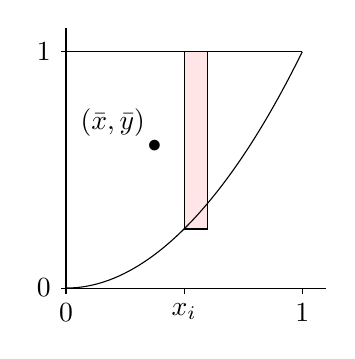
\begin{tikzpicture}[baseline=0,x=3cm,y=3cm]
\fill[fill=red!10] (0.5,0.25) rectangle (0.6,1);
\draw (0.5,0.25) rectangle (0.6,1);
\draw (0,0) -- (1.1,0) ;
\draw (0,0) -- (0,1.1) ;
\foreach \x in {0,1} \draw (\x,0) -- (\x,-2pt) node[anchor=north] {$\x$};
\foreach \y in {0,1} \draw (0,\y) -- (-2pt,\y) node[anchor=east]{$\y$};
\draw (0.5,0) -- (0.5,-2pt) node [anchor=north] {$x_i$};
\node [anchor=south east] at (0.375,0.6) {$(\bar x,\bar y)$};
\node at (0.375,0.6) {$\bullet$};
\draw[color=black] (0,0) parabola (1,1);
\draw (0,1) -- (1,1); 
\end{tikzpicture}
\hskip2cm
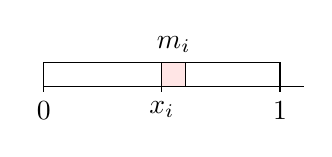
\begin{tikzpicture}[domain=-1.2:1.2,baseline=0,x=3cm,y=3cm]
\fill[fill=red!10] (0.5,0) rectangle (0.6,0.1);
\draw (0,0) -- (1.1,0) ;
\foreach \x in {0,1} \draw (\x,0) -- (\x,-2pt) node[anchor=north] {$\x$};
\draw (0.5,0) -- (0.5,-2pt) node[anchor=north] {$x_i$};
\node[anchor=south] at (0.55,0.1) {$m_i$};
\draw (0,0) rectangle (1,0.1);
\draw (0.5,0) rectangle (0.6,0.1);
\end{tikzpicture}\hfill}}
\caption{Center of mass for a two dimensional plate.}
\label{fig:twodcenterofmass}
\end{figure}

Since the plate has uniform density we may as well assume that
$\sigma=1$. Then the mass of the plate between $\ds x_i$ and $\ds
x_{i+1}$ is approximately $\ds m_i=\sigma(1-x_i^2)\Delta
x=(1-x_i^2)\Delta x$. Now we can compute the moment around the
$y$-axis:
\[M_y=\int_0^1 x(1-x^2)\,dx={1\over4}\]
and the total mass 
\[M=\int_0^1 (1-x^2)\,dx={2\over3}\]
and finally
\[\bar x = {1\over4}{3\over2}={3\over8}.\]
Next we do the same thing to find $\ds \bar y$. The mass of the plate
between $\ds y_i$ and $\ds y_{i+1}$ is approximately $\ds
n_i=\sqrt{y}\Delta y$, so
\[M_x=\int_0^1 y\sqrt{y}\,dy={2\over5}\]
and
\[\bar y={2\over5}{3\over2}={3\over5},\]
since the total mass $M$ is the same. The center of mass is shown in
Figure~\ref{fig:twodcenterofmass}.  
\end{solution}

\begin{example}{Center of Mass under Cosine}{centerofmassundercos}
Find the center of mass of a thin, uniform plate whose shape
is the region between $y=\cos x$ and the $x$-axis between $x=-\pi/2$
and $x=\pi/2$.
\end{example}
\begin{solution}
It is clear that $\ds \bar x=0$, but for practice let's
compute it anyway. We will need the total mass, so we compute it
first:
\[M=\int_{-\pi/2}^{\pi/2} \cos x\,dx=\sin x\Big|_{-\pi/2}^{\pi/2}=2.\]
The moment around the $y$-axis is
\[M_y=\int_{-\pi/2}^{\pi/2} x\cos x\,dx=\cos x+x\sin x\Big|_{-\pi/2}^{\pi/2}=0\]
and the moment around the $x$-axis is
\[M_x=\int_{0}^{1} y\cdot2\arccos y\,dy=\left.y^2\arccos y-{y\sqrt{1-y^2}\over2}+{\arcsin y\over 2}\right|_{0}^{1}={\pi\over4}.\]
Thus
\[\bar x={0\over2},\quad \bar y={\pi\over8}\approx 0.393.\]
\end{solution}


%%%%%%%%%%%%%%%%%%%%%%%%%%%%%%%%%%%%%%%%%%%%
\Opensolutionfile{solutions}[ex]
\section*{Exercises for \ref{sec:centerofmass}}

\begin{enumialphparenastyle}

\begin{ex}
A beam 10 meters long has density $\ds \sigma(x)=x^2$ at
distance $x$ from the left end of the beam. Find the center of mass
$\ds \bar x$.
\begin{sol}
$15/2$
\end{sol}
\end{ex}

\begin{ex}
A beam 10 meters long has density $\sigma(x)=\sin(\pi x/10)$ at
distance $x$ from the left end of the beam. Find the center of mass
$\ds \bar x$.
\begin{sol}
$5$
\end{sol}
\end{ex}

\begin{ex}
A beam 4 meters long has density $\ds \sigma(x)=x^3$ at
distance $x$ from the left end of the beam. Find the center of mass
$\ds \bar x$.
\begin{sol}
$16/5$
\end{sol}
\end{ex}

\begin{ex}
Verify that $\ds\int 2x\arccos x\,dx=
x^2\arccos x-{x\sqrt{1-x^2}\over2}+{\arcsin x\over 2}+C$.
\end{ex}

\begin{ex}
A thin plate lies in the region between $\ds y=x^2$ and the $x$-axis
between $x=1$ and $x=2$. Find the centroid.
\begin{sol}
$\ds \bar x=45/28$, $\ds \bar y = 93/70$
\end{sol}
\end{ex}

\begin{ex}
A thin plate fills the upper half of the unit circle
$\ds x^2+y^2=1$. Find the centroid.
\begin{sol}
$\ds \bar x=0$, $\ds \bar y=4/(3\pi)$
\end{sol}
\end{ex}

\begin{ex}
A thin plate lies in the region contained by $y=x$ and
$\ds y=x^2$. Find the centroid.
\begin{sol}
$\ds \bar x=1/2$, $\ds \bar y=2/5$
\end{sol}
\end{ex}

\begin{ex}
A thin plate lies in the region contained by $\ds y=4-x^2$ and
the $x$-axis. Find the centroid.
\begin{sol}
$\ds \bar x=0$, $\ds \bar y=8/5$
\end{sol}
\end{ex}

\begin{ex}
A thin plate lies in the region contained by $\ds y=x^{1/3}$ and
the $x$-axis between $x=0$ and $x=1$. Find the centroid.
\begin{sol}
$\ds \bar x=4/7$, $\ds \bar y=2/5$
\end{sol}
\end{ex}

\begin{ex}
A thin plate lies in the region contained by 
$\ds \sqrt{x}+\sqrt{y}=1$ and the axes in the first quadrant.
Find the centroid.
\begin{sol}
$\bar x=\bar y=1/5$
\end{sol}
\end{ex}

\begin{ex}
A thin plate lies in the region between
the circle $\ds x^2+y^2=4$ and the circle $\ds x^2+y^2=1$, above the $x$-axis.
Find the centroid.
\begin{sol}
$\ds \bar x=0$, $\ds \bar y=28/(9\pi)$
\end{sol}
\end{ex}

\begin{ex}
A thin plate lies in the region between 
the circle $\ds x^2+y^2=4$ and the circle $\ds x^2+y^2=1$ in the first quadrant.
Find the centroid.
\begin{sol}
$\ds \bar x=\bar y=28/(9\pi)$
\end{sol}
\end{ex}

\begin{ex}
A thin plate lies in the region between 
the circle $\ds x^2+y^2=25$ and the circle $\ds x^2+y^2=16$
above the $x$-axis.
Find the centroid.
\begin{sol}
$\ds \bar x=0$, $\ds\bar y=244/(27\pi)\approx 2.88$
\end{sol}
\end{ex}

\end{enumialphparenastyle}
